% summarize methods, critique, and discuss application

\chapter{Review of the literature}

%?do i need to formalise my literature review? have searched on combos of patient safety machine learning and data mining

\subsection{Patient safety incidents in Health IT}
%Outside of the health context software systems 

\subsubsection{Evidence of harm}
The potential for health IT to support high quality and safe care is well recognized.\cite{Hynes2004}\cite{Bates2003} So, however, is the potential for health IT to introduce new types of error and have unintended consequences.\cite{Harrison2007}\cite{Ash2007}\cite{Campbell2006}

Authors have reported health IT deployment causing harm, and even death.\cite{Han2005} The poor design and usability of some health IT systems has been observed to impact negatively on patient safety, and there have been calls to monitor adverse events due to \gls{EMR} systems.\cite{Johnson2006} \cite{Caldwell2011} \cite{Scott2011} 

Many authors have used qualitative methods to investigate harm occurring to patients that is associated with the use of health IT. Ash et al \cite{Ash2007} administered a structured telephone survey of 176 US hospitals that had computerized physician order entry (CPOE) systems and found that adverse unintended consequences with safety implications were commonly reported by informants. Interestingly, these safety issues seemed to persist throughout the lifespan of the CPOE systems considered, suggesting that in current practice these safety issues are intractable for some reason or another. \label{intractable}

Han et al \cite{Han2005} unexpectedly found a statistically significant increase in paediatric mortality after introduction of CPOE at an academic tertiary-care level children’s hospital. CPOE was introduced at month 13 of an 18 month study period. 1942 children referred and admitted for specialist care during the study period formed the sample. After adjustment for relevant mortality co-variables multivariate analysis revealed that CPOE was independently associated with an increased odds of mortality (odds ratio: 3.28; 95\% confidence interval: (1.94 - 5.55). The authors speculate that this unexpected mortality may be due to impaired communication, delays in the administration of time sensitive medications, and reduced 'face time' with patients resulting from introduction of the CPOE system. However, the mortality-CPOE association discovered can not be used to infer causality, the single research setting considered may not generalize, and the study period after CPOE introduction was short. It is possible that if excess mortality were due to the CPOE introduction this might be a transient 'bedding in' phenomenon.

Scott et al \cite{Scott2011} demonstrated a relationship between health IT user interface design and safety outcomes is a laboratory setting using a within participant design randomized controlled trial and a cohort of 24 junior doctors. Participants performed simulated prescribing tasks with a prototype electronic prescribing system and received modal safety alerts, non-modal safety alerts, or no safety alerts. The primary outcome was prescribing error and error rates varied significantly between experimental arms with modal alerts preventing the most errors. A major limitation of the study is that it occurred in an artificial setting and was limited to simulated clinical scenarios. That this was necessary because it is not currently feasible to carry out such studies ``in the field'' is interesting. It seems highly likely that some software designs will be associated with more or less unintended harm occurring to patients but in routine clinical practice it is not possible to test this or to directly 
improve the design of the software used.


\subsubsection{Response to date}
\label{marketfail}
To date, safety has remained a relatively neglected issue in health IT, it was largely absent as a consideration from the early stages of United Kingdom's national health IT programme \cite{CFHPresentation} and did not feature in the recent US health IT stimulus measures\cite{Hoffman2011}. It has been observed that current market forces are not adequately addressing the potential risks associated with use of health IT.\cite{national2012Health} 

Barriers to improving patient safety in health IT include user disengagement due to a lack of vendor responsiveness,\cite{Shojania2008} contractual barriers, such as non-disclosure and confidentiality clauses, and the absence of a public central repository, or linkages among localised repositories to collect, analyse, and act on safety incidents relating to health IT.\cite{national2012Health}


\subsection{What techniques are used to analyse patient safety incidents?}

\subsubsection{Traditional methods}
Historically, case note review has been the principle method of detecting, and analysing, patient safety events. The seminal paper in this area was a review of 30,195 randomly selected hospital records from 51 New York hospitals which identified 1133 patients (3.7 percent) with disabling injuries caused by medical treatment. The authors classified, and subclassifed, incidents by type into five main categories using a standardized adverse event form. The categories were: \cite{Leape1991} 

\begin{enumerate}
 \item Performance
  \item Prevention
   \item Diagnostic 
    \item Drug treatment 
     \item System
\end{enumerate}


Internationally, an initial first step of human domain-expert classification of incidents according to a taxonomy is the dominant approach adopted in patient safety incident reporting and learning systems.\cite{WHO2005} In the literature this classification then forms the basis of further within category analysis such as qualitative analysis of free text description for a particular category of patient safety incidents to produce a finer taxonomy for classification.\cite{Cassidy2011} Alternatively, initial classification is augmented with targeted free text searches for key words to identify reports of interest. These reports are then categorized and subcategorized by theme. Examples of this approach include Panesar et al's analysis of the free text of all-cause mortality in trauma and orthopaedic surgery\cite{Panesar2012} and Arnot and Smith's analysis of incidents involving neuromuscular blockade. \cite{Arnot2010}


\subsubsection{Data mining techniques in patient safety}
Classifiers have been widely applied to patient safety in a research setting, with mixed results, and are not yet widely used in routine clinical practice.\cite{Bates2003} I could not find an example of clustering being used in the patient safety literature and found only one instance of the related unsupervised machine learning technique, dimensionality reduction, being used.\cite{Bentham2012}

Ong et al used binary classification of incident category to identify incidents as to do with handover or not, and to do with patient identification or not, using \gls{Support Vector Machine} and \gls{Naive Bayes} classifiers. They trained the classifiers using the free text of 600 patient safety incident reports that had been labelled as do with handover or not (300 true, 300 false) and tested on an independent test set containing 372 incident reports (248 true, 124 false). Impressive results for this task were achieved using an SVM: accuracy = 97.98\%, precision = 0.98, recall = 0.98, F-measure = 0.96. However, the validity of this is clearly very limited by the highly selective nature of the data used for testing and this makes the task appear artificial. It is not clear that identifying incidents to do with handover from a sample of incidents with a true:false ratio of 2:1 for being to do with handover or not is a convincing demonstration of the potential utility of automated incident classification.\cite{Ong2010}
  
The identification of new types of adverse drug events has been a hot area of research, possibly due to the large financial stakes in this area. A recent review of studies of the automated detection of adverse drug events in the literature found that data mining techniques can be a useful tool for detecting novel adverse events in large datasets.\cite{Harpaz2012}

Bentham el al. applied unsupervised and supervised \gls{Dimensionality reduction} methods on a \gls{Vector Space Model} with \gls{Term Frequency-Inverse Term Frequency} weighting followed by \gls{Anomaly detection} methods to cluster incidents reported to the NPSA into novel meaningful groups. However the usefulness of this was questionable since they failed to find 'actionable' results. That is they did not identify any new types of incident with common causal factors that were amenable to prevention. \cite{Bentham2012}



\subsection{Previous analysis of patient safety incidents due to computer problems}
\label{litreviewthemes}

\label{bugreportinglit}
Outside of the health setting 'computer problems' due to failure of software are often reported and tracked publicly in a very detailed fashion using specialised software 'bug' reporting and tracking systems. A software bug is an error, flaw, failure, or fault in a computer program or system that produces an incorrect or unexpected result, or causes it to behave in unintended ways\cite{WikipediaBug2013}. 

\begin{figure}[htp]
\centering
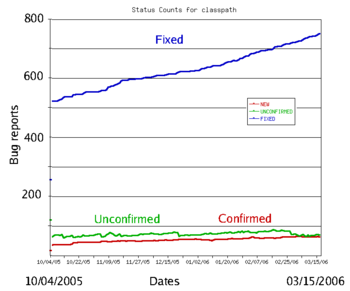
\includegraphics[width=15cm,height=10cm]{figs/bugs2.png}
\label{fig:bugs2}
\caption{The typical bug history (GNU Classpath project data). A new bug submitted by the user is unconfirmed. Once it has been reproduced by a developer, it is a confirmed bug. The confirmed bugs are later fixed. Bugs belonging to other categories (unreproducible, will not be fixed, etc.) are usually in the minority.\cite{WikipediaBug2013}}
\end{figure}

In the health setting public software bug tracking is uncommon but the subset of computer problems which are perceived to impact on patient safety are captured in patient safety reporting and this has been analysed by Magrabi et al.

Magrabi et al analysed 111 patient safety incidents related to computer use across one Australian state to identify `natural categories' for classification.\cite{Magrabi2010} They identified 32 types of computer use problem which they grouped into four main categories:

\begin{enumerate}
 \item Information input (31\%)
 \item Transfer (20\%)
 \item Output (20\%)
 \item General technical (24\%)
\end{enumerate}

Over 50\% of problems were machine related and 45\% were attributed to human–computer interaction. They found that delays in
initiating and completing clinical tasks and the need to redo work were a common result of computer use problems.
\cite{Magrabi2010}

\label{bugreports}

A follow up study of 678 incident reports related to computer use obtained from the US Manufacturer and
User Facility Device Experience (MAUDE) database resulted in the addition of four new categories relating to software use:\cite{Magrabi2012}
\begin{enumerate}
 \item Software functionality
 \item Software system configuration
 \item Software interface with devices
 \item Network configuration
\end{enumerate}

Under-reporting is an issue known to affect all patient safety reporting and learning systems \cite{Shojania2008}\cite{Sari2007} and this limits 
the usefulness of these studies which relied on users reporting incidents. It is possible to capture some types of computer incident, such as unscheduled downtime, in an automated fashion but this was not undertaken in either study.

\subsection{Data mining evaluation criteria}
As discussed previously, evaluation methods in machine learning include objective assessments such as the calculation of a classifier's \gls{accuracy}, \gls{precision}, \gls{recall}, and \gls{F-score}. 

In practice, data mining is evaluated by the usefulness of the insights generated to the organization or individual who invests in it. In the world of business `usefulness' here often means return on investment, and may be quantified objectively on a balance sheet. Within the context of the NPSA patient safety data mining's 'usefulness' refers to the extent to which it is perceived as a helpful tool to the expert patient safety analyst. \cite{Hand2001}\cite{Bentham2012} 

As such unless the outcomes of the data mining process are objectively compared with existing processes, or the data mining process is tied to an intervention which affects a measurable outcome, then objective demonstration of the value of data mining is hard and evaluation is limited to the subjective assessment by domain experts of whether or not value has been added.\cite{Ong2010}\cite{Ong2012}\cite{Bentham2012}


